\title{\textbf{CubeSat Survey}}
\author{
        \textbf{\textit{Miranda Straub, Ryan Watson, John A. Christian, and Jason N. Gross}}\\
        Department of Mechanical and Aerospace Engineering\\
        West Virginia University\\
        Morgantown, WV 26505
}
\date{\today}

\documentclass[11pt]{article}
\usepackage{amsmath}
\usepackage[margin=1.0in]{geometry}
\usepackage{graphicx}
\usepackage{caption}
\usepackage{subcaption}
\usepackage{longtable}

\begin{document}
\maketitle

\begin{abstract}
In recent years, there has been a significant migration towards small satellite missions due to their reduced cost and development time.  Specifically, CubeSats have become increasingly popular not only in university environments, but in government and private industries as well.  The standardization of these 10 cm CubeSats has also allowed for rideshare opportunities, thus finding a launch service provider is much simpler, allowing for more frequent access to space.  CubeSat standards also allow for commercial off the shelf (COTS) hardware components to be made available at reasonable prices, however there is no standard software as of 2014.  NASA Independent Verification and Validation (IV\&V) facility has requested a survey of CubeSats to provide additional insight into all previous CubeSat missions.  This information will assist them in developing a standard software to be used for all future IV\&V CubeSat missions as well as missions at NASA Goddard Space Flight Center (GSFC).
\end{abstract}

\section{Introduction}
The CubeSat Project, developed in 1999 by Professor Jordi Puig-Suari of California Polytechnic State University (Cal Poly), San Luis Obispo and Professor Bob Twiggs of Stanford University's Space Systems Development Laboratory (SSDL), was an initial attempt at standardizing design parameters for small satellites in order to reduce cost and development time.  As a result, these standards have allowed for more frequent launches and therefore easier access to space due to the low-budget nature of CubeSats \cite{CalPoly}.  The CubeSat Project outlines the standards required for CubeSat development while describing specific parameters (i.e. dimensions, mass, deployment mechanisms, etc.) that must be met for the spacecraft to qualify as a CubeSat.  More general information about CubeSats may be found at cubesat.org.

When considering dimensions, a 1U (1 unit) CubeSat must have the dimensions of 10cm x 10cm x 10cm.  Alternate configurations exist and include 2U and 3U CubeSats with dimensions of 10cm x 10cm x 20cm and 10cm x 10cm x 30cm, respectively (see Figure \ref{config}).  In addition to dimensions, mass limitations prohibit CubeSats from exceeding 1.3 kg per unit (U), meaning a 2U CubeSat must not exceed 2.6 kg while a 3U must not exceed 4.0 kg.  These standards also limit the amount of power available for use on the spacecraft.  The specified dimensions pose limitations regarding the surface area available for solar panels.  Previous studies have shown that the average power of a CubeSat can vary from 1W (1U) and 5W (3U).  However, assuming the spacecraft still meets the mass requirements, deployable solar panels can be used to significantly increase the amount of available power (i.e. a 3U CubeSat with deployable panels can have up to 20W of available power) \cite{ClydeSpace}. 

\begin{figure}[ht!]
\centering
\frame{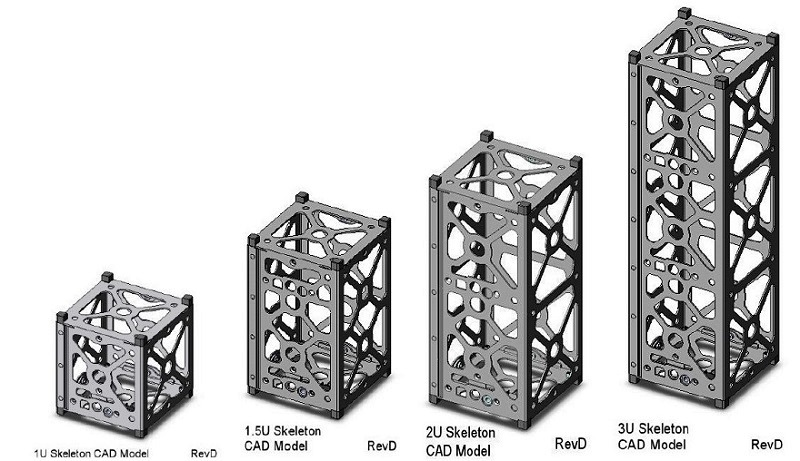
\includegraphics[width=0.75\textwidth]{CubesatConfig}}
\caption{Example of CubeSat Configurations\cite{configimage}}
\label{config}
\end{figure}

CubeSats that meet dimension and mass requirements can be launched from the Poly Picosatellite Orbital Deployer (P-POD) developed by Cal Poly.  The P-POD serves as a standardized deployment system for up to three 1U CubeSats or any equivalent combination.  Any CubeSat being deployed from a P-POD must adhere to additional specific guidelines in the CubeSat Design Specifications document in order to ensure compatibility for a successful deployment.  Some recently proposed experiments, however, have been designed for 6U CubeSat structures, resulting in the need for an alternative deployer.  Fortunately, NASA Wallops, NASA Ames, as well as other institutions have come up with designs for 6U deployers, all of which have been tested and have received a TRL of at least 6 \cite{SmSCTech}.

The standards developed by Cal Poly have resulted in a significant increase in the number of small satellite missions launched over the past few years \cite{MarketAssessment}.  This is partially due to the development of commercial off-the-shelf (COTS) components specifically designed to meet all CubeSat requirements.  Because of this, CubeSats have become relatively inexpensive, making them ideal educational tools in university and classroom settings.  With the development of COTS components, there are a variety of options for various processors and operating systems; however, these options may not always meet the criteria required for various missions.  It is for this reason that NASA IV\&V has been asked to develop a portable, pure software build-and-test system that will provide the capability to develop, debug, and test software on a standard personal computer with no specialized hardware.  Once this is developed, it is expected to be used in collaboration with NASA GSFC's SpaceCube development and testing. 

\section{Methodology}
To determine possible options for a standardized NASA IV\&V software, a comprehensive survey was conducted on past, present, and future CubeSat missions.  This survey initially consisted of all CubeSat missions the research team could find - totalling slightly over 250 missions.  For this particular report, it was decided that the focus would be on domestic missions which narrowed the search to approximately 150 missions, some of which had been launched while others were still only proposed concepts.  This list was consolidated once more to focus on already launched missions as well as missions with launch services confirmed in upcoming years.  
As a result, a comprehensive list of approximately 115 CubeSats has been developed.  

To gather information, the first step involved creating a list of desired mission details.  This information can be categorized as shown in Table \ref{summary}.  A first pass of obtaining data was accomplished by thoroughly searching the internet, although a significant amount of data was left incomplete.  As a second pass, the project managers of each mission were emailed and asked specifically for information regarding data of potential interest to NASA IV\&V as well as any other applicable information or further references.  This helped fill in a significant amount of missing data which was used to create a spreadsheet that will be provided electronically upon delivery of this report and includes all data collected in the categories described in Table \ref{summary}.

It should be noted that despite all efforts made in this project, the results of this survey only provide estimates used to identify trends in the presented data.  For example, many of the surveyed missions were conducted by universities with limited budgets while others were sponsored by private companies or government agencies with higher budgets.  This should be considered when analyzing numerical data obtained from this survey and will hopefully be made prominent through the discussion of results. 

\begin{table}[h]
\small
\centering
\caption{Summary of Data Collected for CubeSat Survey}
\label{summary}
\begin{tabular}{|l|l|l|}
\hline
\textbf{Mission Information} & \textbf{Launch Information} & \textbf{IV\&V Information} \\ \hline
Name of Satellite & Launch Date & Processor \\ \hline
Mission Objective & Launch Vehicle/Mission & Orbit \\ \hline
Sponsor & Mission Status & Uplink/Downlink \\ \hline
Manufacturer & Deployer & Attitude Determination \\ \hline
Domestic & Program & Attitude Control \\ \hline
Size & Orbit Parameters & Orbit Determination \\ \hline
Mass &  & Miscellaneous \\ \hline
\end{tabular}
\end{table}

\section{Results of Survey \& Discussion}
\subsection{Analysis of CubeSat Market and Survey Sample Set}
A market assessment conducted by SpaceWorks Enterprises, Inc. in 2014 showed that of the nanosatellites launched between 2009 and 2013, 47\% can be categorized as 1U CubeSats \cite{MarketAssessment}.  Although not enough information is given to determine how many 2U and 3U CubeSats have been launched, there seems to be a significant trend towards 3U CubeSat missions based on the information in Figure \ref{peryear}.  These results show the increase in overall CubeSat missions and gives reason to believe this trend will continue in the near future.

\begin{figure}[h]
\centering
\frame{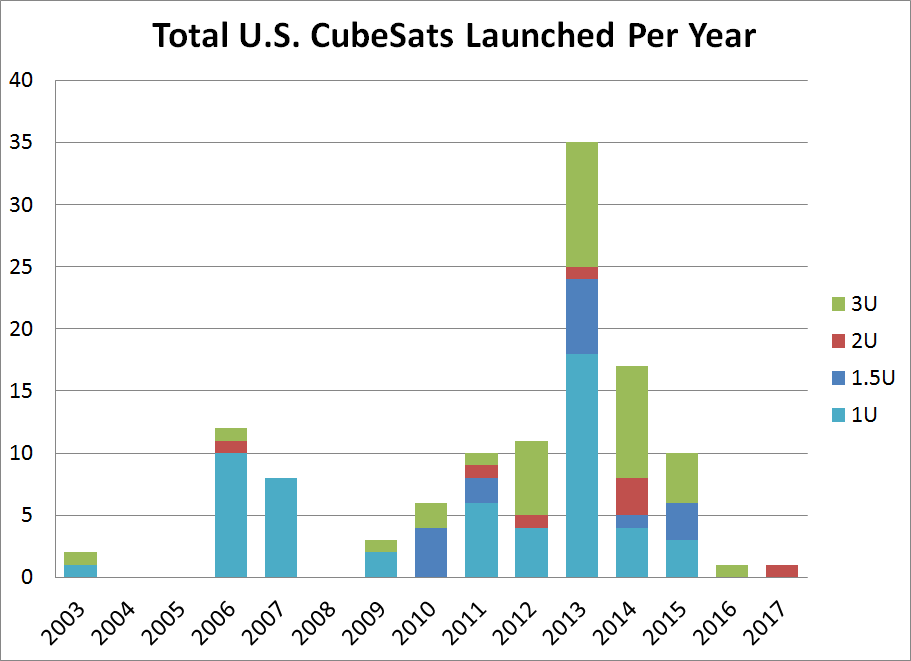
\includegraphics[width=0.75\textwidth,trim=0.1in 0.1in 0.1in 0.1in,clip]{Bar_SizeYear}}
\caption{Results of survey showing the size and number of CubeSats launched per year as of August 2014 (based on 116 CubeSats with applicable data)}
\label{peryear}
\end{figure}

Figure \ref{classperyear} shows the total number of U.S. CubeSats launched per year, divided by class (i.e. private, government, university, military, etc.).  From this graph, it is evident that a majority of launches have been for university missions and educational purposes;  however there has been a significant increase seen in government missions as well as privately funded missions.  

\begin{figure}[ht!]
\centering
\frame{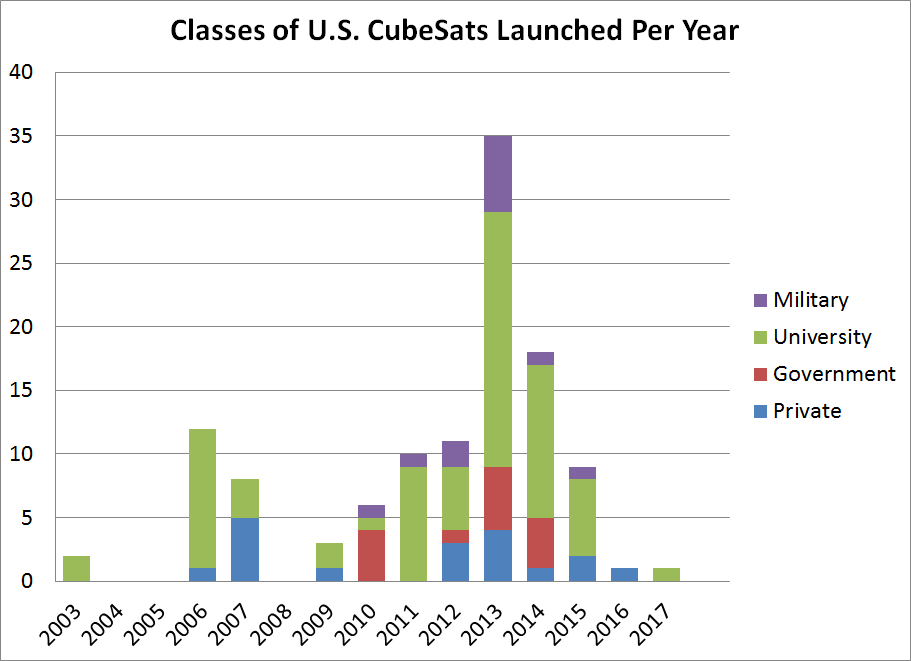
\includegraphics[width=0.75\textwidth,trim=0.1in 0.1in 0.1in 0.1in,clip]{Bar_Classes}}
\caption{Results of survey showing the number of U.S. CubeSats launched per year, divided by class, as of August 2014 (based on 116 CubeSats with applicable data)}
\label{classperyear}
\end{figure}

\begin{figure}[h!]\label{pieclasses}
    \centering
    \begin{subfigure}[t]{0.5\textwidth}
        \centering
        \frame{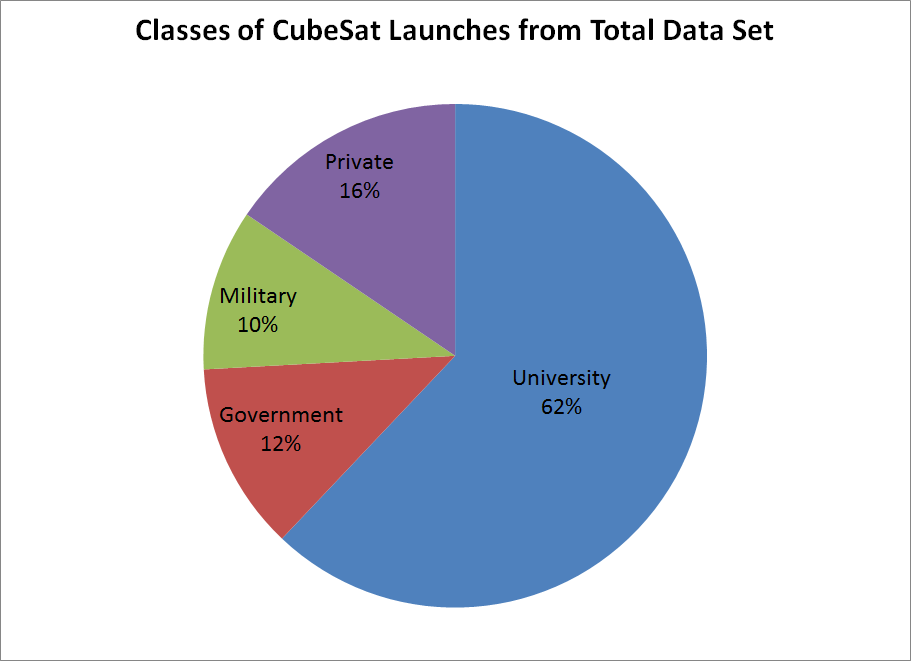
\includegraphics[height=2in,trim=0.1in 0.1in 0.1in 0.1in,clip]{Pie_Total}}
        \caption{Results from Total Data Set}
    \end{subfigure}%
    ~ 
    \begin{subfigure}[t]{0.5\textwidth}
        \centering
        \frame{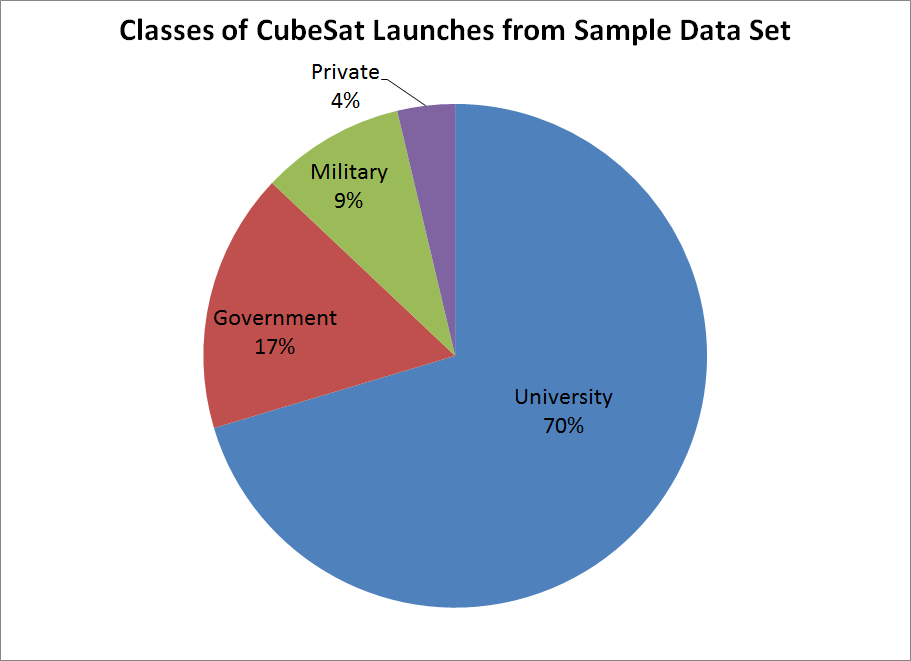
\includegraphics[height=2in,trim=0.1in 0.1in 0.1in 0.1in,clip]{Pie_Sample}}
        \caption{Results from Sample Data Set}
    \end{subfigure}
    \caption{Comparison of CubeSat class percentages based on data from all information collected and the sample set in which processor information was known.}
\end{figure}

Since the collected data providing processor information does not encapsulate the total CubeSat data set, it is important to point out that data may be skewed.  It was believed that a majority of collected data came from university missions due to the missions being largely educational with project managers willing to provide information to other organizations.  Military and government missions are more likely to be less available due to various restrictions which also would cause results to encompass mostly university missions.  However, upon further investigation, it was found that the sampled data set was similar to that total data set as seen in Figures 4 and \ref{compare}. 

\begin{figure}[ht!]
\centering
\frame{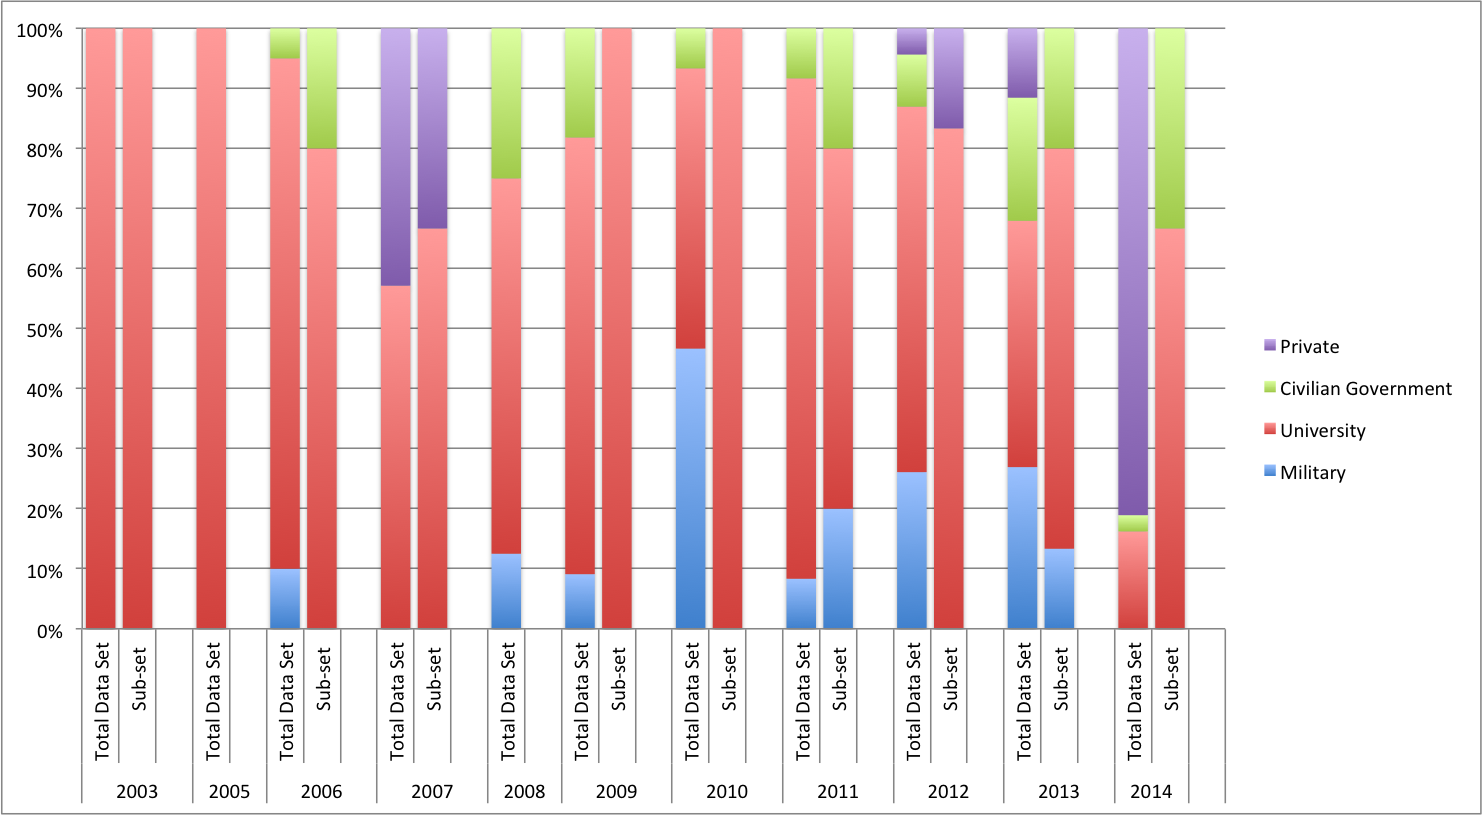
\includegraphics[width=0.75\textwidth,trim=0.1in 0.1in 0.1in 0.1in,clip]{DataComparison}}
\caption{Bar graph visualization comparing classes from total data set and sampled data set}
\label{compare}
\end{figure}

\subsection{Flight Processors}
For this report, it is assumed that processors and operating systems are of most importance to NASA IV\&V.  This will provide insight into which processors are most popular within the CubeSat community and will allow IV\&V to develop approaches with the widest possible impact.  Based on the 55 missions where processor data was attainable, almost 40\% of these missions utilized PIC processors.  Of these processors, 52\% used the PIC18.  These results are summarized in Figure \ref{processors}.  Upon further investigation, it was concluded that 90\% of the PIC18 processors were used in 1U missions.  Table \ref{list} in the Appendix shows an abbreviated list of CubeSat missions sorted by size to show the trend of processors used.  It is also important to note that Pumpkin currently provides Pluggable Processor Modules (PPM) available with their CubeSat Kit and is capable of incorporating the following processors into the flight module:  SiLabs C805, PIC24, PIC33, and TI MSP430.  The convenience of purchasing processors with a Pumpkin CubeSat Kit may play a key role in processor trends, especially for 1U CubeSats, although many factors were not accounted for in this analysis (i.e. budget, development time, cost of materials, etc.) and  could have played a key role in determining the processors as well.

\begin{figure}[h!]
    \centering
    \begin{subfigure}[t]{0.5\textwidth}
        \centering
        \frame{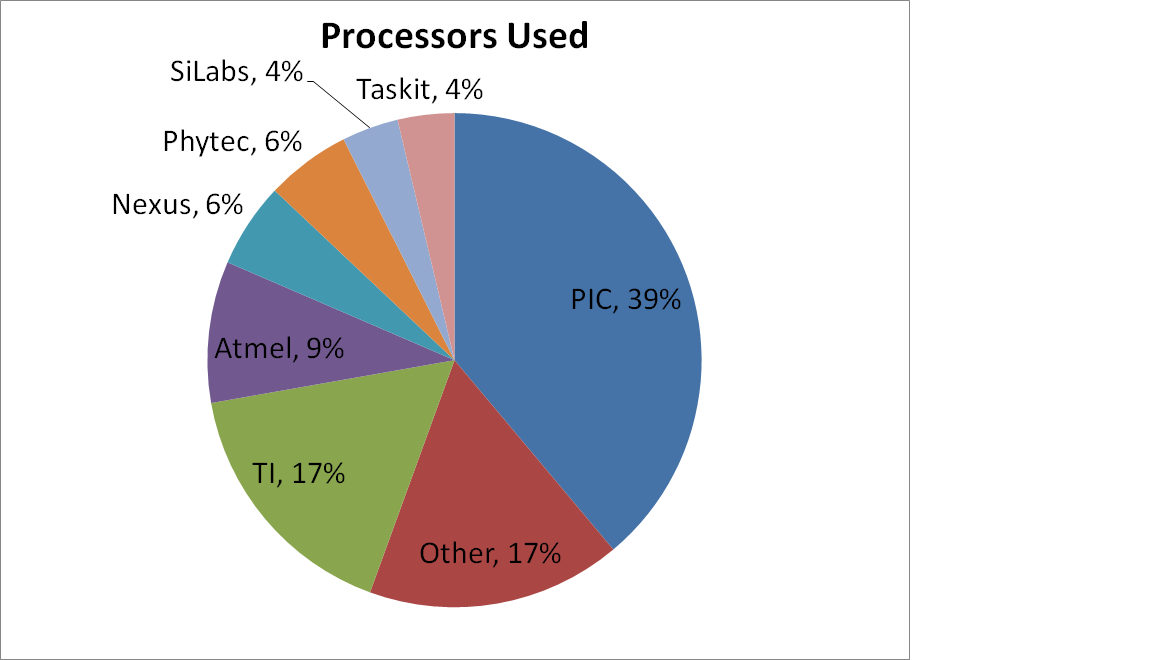
\includegraphics[height=2in,trim=0.1in 0.1in 0.1in 0.1in,clip]{Pie_Processors}}
        \caption{Summary of processors used (Total: 55)}
    \end{subfigure}%
    ~ 
    \begin{subfigure}[t]{0.5\textwidth}
        \centering
        \frame{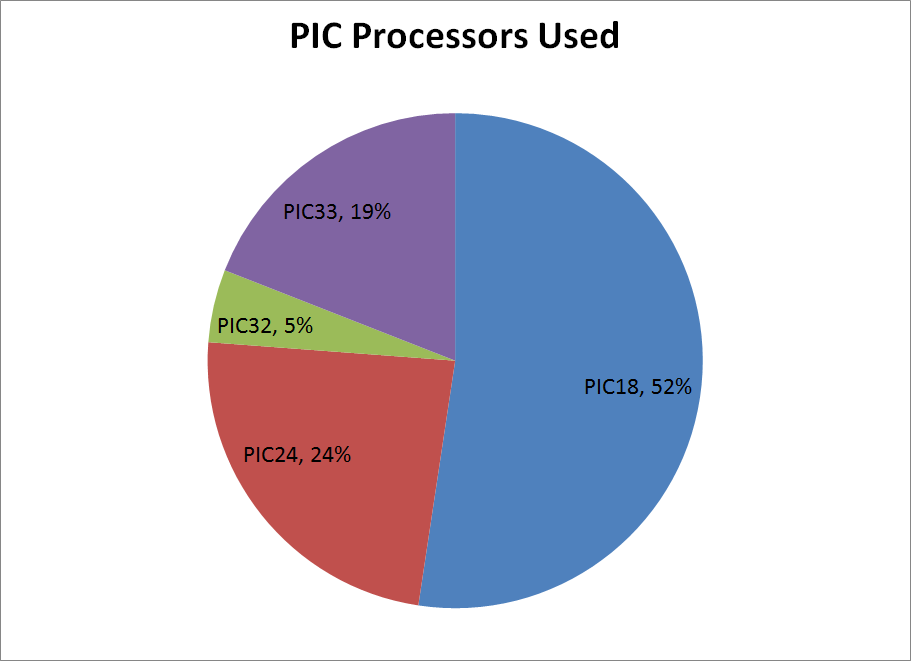
\includegraphics[height=2in,trim=0.1in 0.1in 0.1in 0.1in,clip]{Pie_PIC}}
        \caption{Breakdown of PIC processors used (Total: 21)}
    \end{subfigure}
    \caption{Summary of processors used in CubeSats}
		\label{processors}
\end{figure}

To counter the potential skewness presented by the large percentage of university missions when considering processors, Figure \ref{nonuniv} shows the percentage of processors used on all non-university missions.  However, the results were once again consistent such that PIC processors totaled over 50\% of all processor data recorded.
 
\begin{figure}[ht!]
\centering
\frame{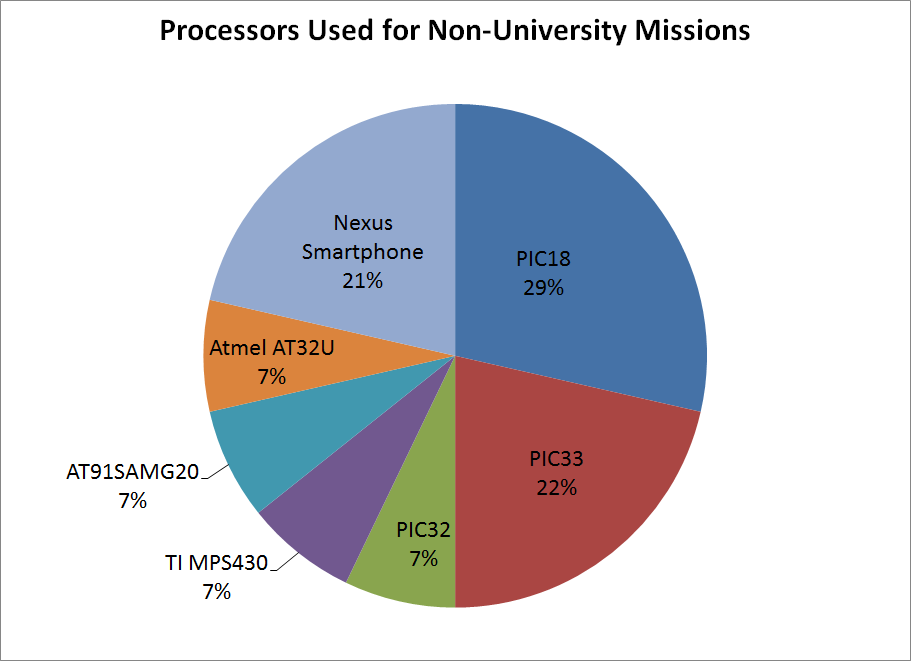
\includegraphics[width=0.75\textwidth,trim=0.1in 0.1in 0.1in 0.1in,clip]{nonuniv}}
\caption{Results of survey showing the processors used for non-university missions (Total: 14)}
\label{nonuniv}
\end{figure}

\subsection{Operating Systems}
Salvo and Linux were the two most commonly used operating systems in the CubeSat missions surveyed.  Salvo is available with the purchase of any Pumpkin PPM and is included with the purchase of a Pumpkin CubeSat Kit.  Most processors provide various options for programming and therefore no concrete conclusion can be made as to which operating system should be used by IV\&V.

\begin{figure}[h !]
\centering
\frame{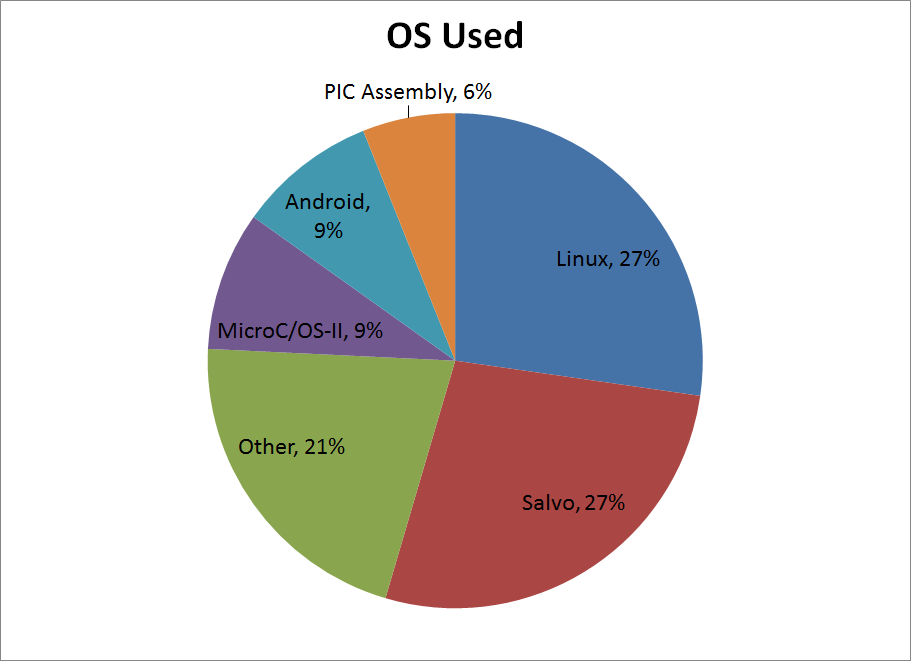
\includegraphics[width=0.75\textwidth,trim=0.1in 0.1in 0.1in 0.1in,clip]{Pie_OS}}
\caption{Results of survey showing the percentage of OS used in CubeSat missions (Total: 33)}
\label{OS}
\end{figure}

\subsection{Discussion}
Based on the information collected from this survey, a majority of CubeSat missions have used PIC processors (specifically PIC18) with either Linux or Salvo operating systems.  The availability of Pumpkin CubeSat kits is likely a major contributor to these results, although this was not confirmed in this survey.  As mentioned before, the results of this survey do not take into consideration factors such as budget, time constraints, component availability, etc. so it is our recommendation that NASA IV\&V use their previous knowledge and experience with processors and operating systems to create their own verification and validation software.  Some crucial aspects to consider when choosing a processor are cost, user interface, and power requirements, each of which will be determined by the nature of the mission.  In addition, it is worth noting that the results of this survey lead us to believe that successful missions can be achieved through the use of PIC processors and Linux or Salvo operating systems.  Electronically attached to this report are data sheets for the processors used in this survey.

\begin{table}[h]
\centering

\caption{Processor Specifications}
\label{procspecs}
\resizebox{\textwidth}{!}{
\begin{tabular}{|c|c|c|c|}
\hline
\textbf{Processor} & \textbf{Max. Operating Frequency (MHz)} & \textbf{Max. Program Memory (KB)} & \textbf{Clock Speed} \\ \hline
PIC18 & 40 & 32 & 32 kHz \\ \hline
PIC24 & 32 & 256 & 32 kHz \\ \hline
PIC32 & 50 & 256 & 32 kHz \\ \hline
PIC33 & 16 & 536 & 32 kHz \\ \hline
TI MPS430 & 24 & 512 & 32 kHz \\ \hline
SiLabs 8051 & 50 & 32 & 16 MHz \\ \hline
Freescale HC12 & 50 & 512 & 32 kHz \\ \hline
Atmel AtxMega & 32 & 128 & 32 kHz \\ \hline
Atmel AT91SAM9 & 210 & 8 & 32 kHz \\ \hline
Phytec phyCORE-LPC3250 & 208 & 32 & 13 MHz \\ \hline
Taskit Stamp9G20 & 396 & 32 & 32 kHz \\ \hline
\end{tabular}
}
\end{table}

\section{Future Work}
Evident in the NASA's FY 2015 budget request is the agency's near-term interest in CubeSats. The requested 2015 NASA budget indicates a \$25M allocation to CubeSat projects over the next five years \cite{budget}. In light of this, there are currently multiple open or future planned solicitations accepting CubeSat based mission proposals. In particular, a review of the NSPIRES website (nspires.nasaprs.com), shows at least three specific solicitations that request CubeSat proposals, listed in Table \ref{future}. 

In addition to the \$25M line-item, NASA Earth Science Technology Office (ESTO) funds missions to validate technology through its In-Space Validation of Earth Science Technologies (InVEST) program. Currently InVEST is planning to spend \$13M over four years on four 3U CubeSat missions \cite{klumpar}. One mission currently in development is ICECUBE or Earth-1, which is being built at Goddard Space Flight Center. 

\begin{table}[h]
\caption{CubeSat Proposal Opportunities}
\label{future}
\centering
\resizebox{\textwidth}{!}{
\begin{tabular}{|p{2.0in}|l|p{5.0in}|}
\hline
\multicolumn{3}{|c|}{\textbf{CubeSat Proposal Opportunities}} \\ \hline
\multicolumn{1}{|c|}{\textbf{Name}} & \multicolumn{1}{c|}{\textbf{Solicitation Number}} & \multicolumn{1}{c|}{\textbf{Description}} \\ \hline
Remote Sensing Theory for Earth Science & NNH14ZDA001N-RST & Remote sensing science to establish a theoretical basis for measuring Earth surface properties using reflected, emitted, and scattered electromagnetic radiation and to develop the methodologies and technical approaches to analyze and interpret such measurements lies at the heart of NASA’s mission. \\ \hline
Heliophysics Technology and Instrument Development for Science & NNH13ZDA001N-HTIDS & The H-TIDeS program solicits proposals for investigations that are relevant to NASA's programs in Heliophysics. \\ \hline
Astrophysics Research and Analysis Program & NNH13ZDA001N-APRA & The Astrophysics Research and Analysis Program (APRA) program solicits basic research proposals for investigations that are relevant to NASA's programs in astronomy and astrophysics and includes research over the entire range of photons, gravitational waves, and particle astrophysics. \\ \hline
Smallsat Technology Partnership & NNA13ZUA001C & NASA has selected 13 university teams for collaborative projects to develop and demonstrate new technologies and capabilities and spur innovation in communication, navigation, propulsion, science instruments, and advanced manufacturing for small spacecraft. \\ \hline
Human Exploration and Operations Mission Directorate & NNH14HEOMD001L & Proposed CubeSat investigations must address an aspect of science, technology development, education, or operations encompassed by NASA’s strategic goals and outcomes as identified in the NASA Strategic Plan. \\ \hline
Spacecraft Operating Software System in Support of CubeSat Vault Electronics & NNL14518620Q & NASA/LARC has a requirement for Spacecraft Operating Software System in support of CubeSat Vault Electronics. \\ \hline
Opportunity Notice to Participate in ITS Centennial Challenges Program as an Allied Organization for Small Spacecraft Challenges & NNH14STMD005L & Organizations may submit proposals for consideration as either Lead Allied Organization or Supporting Allied Organization for CubeSat based Centennial Challenge. \\ \hline
\end{tabular}
}
\end{table}

Further, NASA’s interest in the future of CubeSats is evidenced in its plans to host a CubeSat based Centennial Challenge competition in order to spur the advancement of propulsion and communication technologies for deep space applications. Primarily, the challenge is designed to develop innovative ways to return error free data from deep space without government assistance, and to demonstrate lunar orbital plane change from equatorial to polar \cite{solicitation}. This Centennial challenge will inevitably lead to technology and knowledge that will advance the field beyond its current state. NASAs investment in this event demonstrates the agency’s commitment to the field. 

NASA is showing a great commitment to the use of CubeSats for rigorous scientific endeavors as demonstrated by the availability of funding opportunities and the development of a CubeSat Centennial Challenge. 

\newpage
\section{Appendix}

\begin{center}
\begin{longtable}{|l|l|l|l|l|}
\caption{Abbreviated summary of CubeSat missions grouped by size, displaying launch date, processor used, and operating system used} 
\label{list} \\

\hline \multicolumn{1}{|c|}{\textbf{Name of Satellite}} & \multicolumn{1}{c|}{\textbf{Size}} & \multicolumn{1}{c|}{\textbf{Launch Date}} & \multicolumn{1}{c|}{\textbf{Processor}} & \multicolumn{1}{c|}{\textbf{OS}}\\ \hline 
\endfirsthead

\multicolumn{5}{c}%
{{\bfseries \tablename\ \thetable{} -- continued from previous page}} \\
\hline \multicolumn{1}{|c|}{\textbf{Name of Satellite}} &
\multicolumn{1}{c|}{\textbf{Size}} &
\multicolumn{1}{c|}{\textbf{Launch Date}} &
\multicolumn{1}{c|}{\textbf{Processor}} &
\multicolumn{1}{c|}{\textbf{OS }} \\ \hline 
\endhead

\hline \multicolumn{5}{|r|}{{Continued on next page}} \\ \hline
\endfoot

\hline \hline
\endlastfoot
TUSat1 & 1U & 2003 & i80386 & DOS 3.0 \\ \hline
CP-1 & 1U & 7/26/2006 & PIC18 & Not Supplied \\ \hline
CP-2 & 1U & 7/26/2006 & PIC18 & Not Supplied \\ \hline
MEROPE & 1U & 7/26/2006 & HCS12 & C \\ \hline
CP-3 & 1U & 4/17/2007 & PIC18 & Not Supplied \\ \hline
CP-4 & 1U & 4/17/2007 & PIC18 & Not Supplied \\ \hline
MAST & 3x1U & 4/17/2007 & PIC18 & Not Supplied \\ \hline
CP-6 & 1U & 5/19/2009 & PIC18 & Not Supplied \\ \hline
Explorer-1 Prime 2 (HRBE) & 1U & 10/28/2011 & HCS12 & Not Supplied \\ \hline
MCubed/COVE & 1U & 10/28/2011 & Stanp9G20 & Linux \\ \hline
CP-5 & 1U & 9/13/2012 & PIC18 & Not Supplied \\ \hline
PhoneSat v1a (Graham) & 1U & 4/21/2013 & HTC & Android 2.3.3 \\ \hline
PhoneSat v1b (Bell) & 1U & 4/21/2013 & HTC & Android 2.3.3 \\ \hline
PhoneSat v2.0 (Alexander) & 1U & 4/21/2013 & Samsung & Android 2.3.3 \\ \hline
COPPER & 1U & 11/19/2013 & PIC24 & Not Supplied \\ \hline
UAH/ChargerSat-1 & 1U & 11/19/2013 & ATxmega128A1U & Atmel Studio \\ \hline
SwampSat & 1U & 11/19/2013 & TI MSP430 & Not Supplied \\ \hline
KySat-2 & 1U & 11/19/2013 & SiLabs 8051 & Not Supplied \\ \hline
Trailblazer & 1U & 11/19/2013 & Pumpkin & Salvo \\ \hline
DragonSat-1 & 1U & 11/19/2013 & PIC33 & Salvo \\ \hline
Lunar Orbiter/Lander CubeSat & 1U & 11/19/2013 & TI MSP430 & SPARK \\ \hline
NPS-SCAT & 1U & 11/19/2013 & TI MSP430 & Salvo \\ \hline
CP-8/IPEX & 1U & 12/6/2013 & AT91SAM9 & Linux \\ \hline
MCubed/COVE 2 & 1U & 12/6/2013 & Stamp9G20 & Linux \\ \hline
DICE & 2x1.5U & 10/28/2011 & TI MSP430 & Salvo \\ \hline
FIREBIRD 1A & 2x1.5U & 12/6/2013 & PIC24 & Salvo \\ \hline
FIREBIRD 1B & 2x1.5U & 12/6/2013 & PIC24 & Salvo \\ \hline
PSAT & 2x1.5U & 2015 & basicStamp & basic \\ \hline
BRICSat-P & 1.5U & 2015 & PIC33 & Salvo \\ \hline
ION & 2U & 7/26/2006 & SH2 & SID \\ \hline
PSSC-2 & 2U & 7/8/2011 & PIC18 & PIC Assembly \\ \hline
CXBN & 2U & 9/13/2012 & TI MPS430 & Not Supplied \\ \hline
LMRSat & 2U & 2014 & TI MPS430 & Salvo \\ \hline
CP-9 & 2U & TBA & AT91SAM9 & Linux \\ \hline
QuakeSat & 3U & 6/30/2003 & i80486 & Linux \\ \hline
GeneSat-1 & 3U & 12/16/2006 & PIC & C++ \\ \hline
RAX-1 & 3U & 11/19/2010 & TI MPS430 & Not Supplied \\ \hline
RAX-2 & 3U & 10/28/2011 & TI MPS430 & Not Supplied \\ \hline
CINEMA 1 & 3U & 9/13/2012 & PIC33 & Not Supplied \\ \hline
CSSWE & 3U & 9/13/2012 & TI MPS430 & Salvo \\ \hline
Aeneas & 3U & 9/13/2012 & PIC24 & Not Supplied \\ \hline
ALL-STAR/THEIA & 3U & 4/18/2014 & AT32UC3A3256S & Not Supplied \\ \hline
KickSat & 3U & 4/18/2014 & TI CC430 & Not Supplied \\ \hline
SporeSat & 3U & 4/18/2014 & PIC32 & uC/OS-II \\ \hline
INSPIRE & 3U & 2014 & AT91SAM9 & Not Supplied \\ \hline
RACE & 3U & 2014 & LPC3250 & Linux \\ \hline
RAVAN & 3U & 2015 & SiLabs 8051 & Not Supplied \\ \hline
ARMADILLO & 3U & 2015 & LPC3250 & Linux \\ \hline
USS Langley & 3U & 2015 & PIC33 & Salvo \\ \hline
CP-10/EXOCUBE & 3U & 2015 & AT91SAM9 & Linux \\ \hline
Bevo-2 & 3U & TBA & LPC3250 & Linux \\ \hline
\end{longtable}
\end{center}

\bibliographystyle{aiaa}
\bibliography{CubeSatReferences}
\end{document}
